\paragraph{QuizziPedia::Front-End::ModelViews::StatisticsModelView}

\label{QuizziPedia::Front-End::ModelViews::StatisticsModelView}

\begin{figure}[ht]
	\centering
	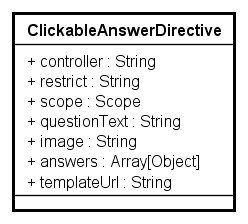
\includegraphics[scale=0.5,keepaspectratio]{UML/Classi/Front-End/QuizziPedia_Front-end_Templates_ClickableAnswerTemplate.png}
	\caption{QuizziPedia::Front-End::ModelViews::StatisticsModelView}
\end{figure} \FloatBarrier

\begin{itemize}
	\item \textbf{Descrizione}: classe di tipo modelview la cui istanziazione è contenuta all'interno della variabile di ambiente \$scope di \textit{Angular.js\ped{G}}. All'interno di essa sono presenti le variabili e i metodi necessari per il \textit{Two-Way Data-Binding\ped{G}} tra la view \texttt{UserView} e il controller \texttt{StatisticsController};
	\item \textbf{Utilizzo}: viene utilizzata per effettuare il \textit{Two-Way Data-Binding\ped{G}} tra la view \texttt{UserView} e il controller \texttt{StatisticsController} rendendo disponibili variabili e metodi;
	\item \textbf{Relazioni con altre classi}: 
	\begin{itemize}
		\item \textit{IN} \texttt{UserView}: view contenente le direttive dei dati personali dell'utente, delle sue statistiche relative ai questionari e agli allenamenti effettuati e dei questionari a cui è iscritto; 
		\item \textit{IN} \texttt{StatisticsController}: questa classe permette di le statistiche di un utente;
	\end{itemize}
	\item \textbf{Attributi}: 
	\begin{itemize}
		\item ;
	\end{itemize}
	\item \textbf{Metodi}: 
	\begin{itemize}
		\item \texttt{+} \texttt{getStatistics(username: String)} \\ 
		Metodo che permette di ottenere le statistiche si un utente grazie all'utilizzo di \texttt{StatisticsService}; \\
		\textbf{Parametri}: 
		Metodo costruttore della classe. \\
		\begin{itemize}
			\item \texttt{username: String} \\
			Parametro contenente la stringa username utilizzata per poter recuperare le giuste statistiche attraverso lo \texttt{StatisticsService}; 
		\end{itemize}
	\end{itemize}
\end{itemize}	

